\documentclass[11pt]{article}  
\usepackage[margin=1in]{geometry}
\parindent=0in
\parskip=8pt
\usepackage{fancyhdr,amssymb,amsmath, graphicx, listings,float,subfig,enumerate,epstopdf,color,multirow,setspace,bm,textcomp}
\usepackage[usenames,dvipsnames]{xcolor}
\usepackage{hyperref}
\usepackage{graphicx}
\graphicspath{{./Images}}

\pagestyle{fancy}


\begin{document} 

\lhead{Assignment \# 2}
\chead{Robert Denim Horton}
\rhead{\today}

\begin{center}\begin{Large}
CS 4720/5720 Design and Analysis of Algorithms

Homework \#2

Student: (Robert Denim Horton)
\end{Large}
\end{center}

\section*{Answers to homework problems:}

\begin{center}
	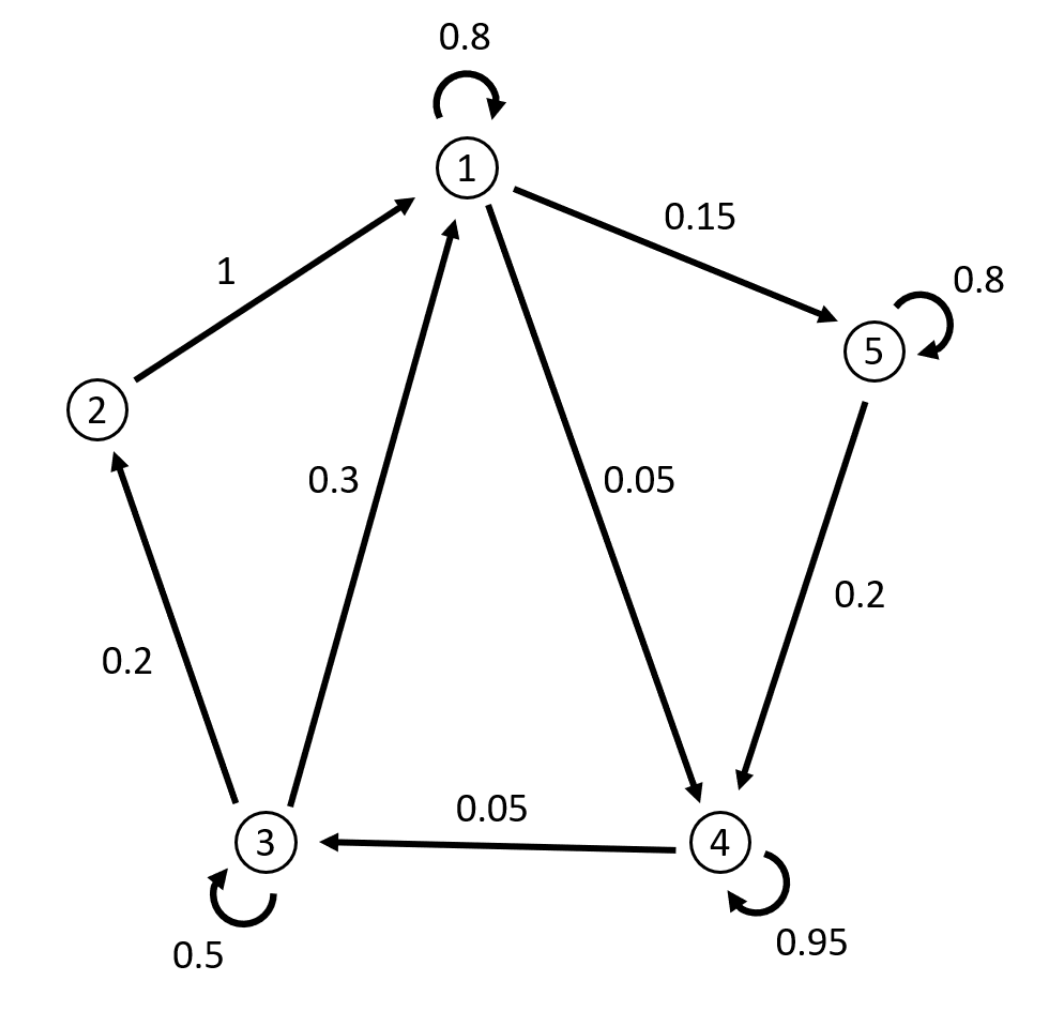
\includegraphics[scale=0.8]{Figure1.1}\\
	Figure 1.1
\end{center}

% Question 1
\begin{enumerate}
	\item Let every node's population be 1 (i.e., $N_i = 1$  for each i). Let  $\beta = 0.8$ and $\gamma = 0.5$. Let all initial infections be 0 except for node 1; node 1's initial infection should be 0.01 (so  $I_i(0)=0.01$ and $S_i(0)=0.99$ , but all other nodes have $S_i(0)=1$,  $I_i(0) = 0$ and $R_i(0) = 0$). What are the S, I, and R quantities after 1 time step?
\end{enumerate}
% Question 1 Answers
\textcolor{gray}{
Answers:
\begin{enumerate}
		\item Quickly formalizing our network as shown in Figure 1.1 we consider each node to represent a group of people that have different fractions of the people at node $i$ as either susceptible ($S_i(t)$), infectious ($R_i(t)$), or recovered ($I_i(t)$). In class we were also given equations to help apply and track these percentages through each time step, $t$ So we get the following equations below.
\begin{align*}
	S_i(t+1) 	&=  S_i(t) - \left(\frac{\beta \times a_{ij} \times S_i(t) \times I_i(t)}{N_i}\right) \\
	I_i(t+1) 	&=  I_i(t) + \left(\frac{\beta \times a_{ij} \times S_i(t) \times I_i(t)}{N_i}\right) - (\gamma I_i(t)) \\
	R_i(t+1) 	&=  R_i(t) + \big(\gamma \times I_i(t)\big) \\
\end{align*}
We further defined the equations to have practical applications on networks by defining the part in red as the summation of each of the $i_{th}$ rows and for this problem we know the population at each node is 1 ($N_i=1$). So we get,
\begin{align*}
	S(t+1) 	&=  S(t) - \beta S(t)_{diag} AI(t) \\
	I(t+1) 	&=  I(t) + \beta S(t)_{diag}AI(t) - (\gamma I(t)) \\
	R(t+1) 	&=  R(t) + \big(\gamma \times I(t)\big) \\
\end{align*}
In early lectures we learned how to represent networks as an adjacent matrix where each row represent a single node with values along the columns representing the edges coming from that node to other corresponding column nodes.  So this network can be represented as the adjacent matrix, $A$, below.\\
\begin{center}
	$A=\begin{bmatrix} 
		0.8  & 0.0 & 0.0 & 0.05 & 0.15 \\
		1.0  & 0.0 & 0.0 & 0.0   & 0.0 \\
		0.3  & 0.2 & 0.5 & 0.0 & 0.0 \\
		0.0  & 0 .0 & 0.05 & 0.95 & 0.0 \\
		0.0  & 0 .0 & 0.0 & 0.2 & 0.8 \\
	\end{bmatrix}$\\
\end{center}
We also defined a matrix, of the same size (filled with 0.0 except along the diagonal), where the values for each node $S(t)$ at time step $t$ is stored along the diagonal of this matrix which is denoted as  $S(t)_{diagonal}$ \textcolor{red}{ which is essentially the probability of each node getting infected through the spreading of the disease to another node}. This matrix is defined below specifically for this problem.\\
\begin{center}
 	$S(t)_{diag}=\begin{bmatrix} 
		S_1(t)  & 0.0 & 0.0 & 0.0 & 0.0 \\
		0.0  & S_2(2) & 0.0 & 0.0   & 0.0 \\
		0.0  & 0.0 & S_3(t) & 0.0 & 0.0 \\
		0.0  & 0 .0 & 0.0 & S_4(t) & 0.0 \\
		0.0  & 0 .0 & 0.0 & 0.0 & S_5(t) \\
	\end{bmatrix}$
\end{center}
Now formalizing the network at time step 0, we can define the populations percentages amongst nodes as row-vectors where each column in the row represents the different percentages at that node.  So for this equation we get\\
\begin{center}
 	$S(0)=\begin{bmatrix} 
		0.99  &
		1.0  &
		1.0  &
		1.0 &
		1.0  &
	\end{bmatrix}$\\
 	$I(0)=\begin{bmatrix} 
		0.01  &
		0.0  &
		0.0  &
		0.0  &
		0.0  &
	\end{bmatrix}$\\
 	$R(0)=\begin{bmatrix} 
		0.0  &
		0.0  &
		0.0  &
		0.0  &
		0.0  &
	\end{bmatrix}$\\
\end{center}
Now, to solve the percentage for each nodes populations for time step $t=1$ we can code this into a quick python program to perform dot and matrix multiplication to help check our work and further exploration into this network for further problems.  For this problem we will do the first equation to show understanding of the process.  First we want to solve for S(1), so\\
\begin{align*}
	S(1) &=
		\begin{bmatrix} 
		0.01 &
		0.0 	&
		0.0 	&
		0.0 	&
		0.0 	&
		\end{bmatrix}
		 - 0.8 
		\begin{bmatrix} 
		0.99  & 0.0 & 0.0 & 0.0 & 0.0 \\
		0.0  & 1.0 & 0.0 & 0.0   & 0.0 \\
		0.0  & 0.0 & 1.0 & 0.0 & 0.0 \\
		0.0  & 0 .0 & 0.0 & 1.0 & 0.0 \\
		0.0  & 0 .0 & 0.0 & 0.0 & 1.0 \\
		\end{bmatrix}
		\begin{bmatrix} 
		0.8  & 0.0 & 0.0 & 0.05 & 0.15 \\
		1.0  & 0.0 & 0.0 & 0.0   & 0.0 \\
		0.3  & 0.2 & 0.5 & 0.0 & 0.0 \\
		0.0  & 0 .0 & 0.05 & 0.95 & 0.0 \\
		0.0  & 0 .0 & 0.0 & 0.2 & 0.8 \\
		\end{bmatrix}
		\begin{bmatrix} 
		0.01 \\
		0.0 	\\
		0.0 	\\
		0.0 	\\
		0.0 	\\
		\end{bmatrix}\\
&=
		\begin{bmatrix} 
		0.01 &
		0.0 	&
		0.0 	&
		0.0 	&
		0.0 	&
		\end{bmatrix}
		 - 
		\begin{bmatrix} 
		0.72  & 0.0 & 0.0 & 0.0 & 0.0 \\
		0.0  & 0.8 & 0.0 & 0.0   & 0.0 \\
		0.0  & 0.0 & 0.8 & 0.0 & 0.0 \\
		0.0  & 0 .0 & 0.0 & 0.8 & 0.0 \\
		0.0  & 0 .0 & 0.0 & 0.0 & 0.8 \\
		\end{bmatrix}
		\begin{bmatrix} 
		0.8  & 0.0 & 0.0 & 0.05 & 0.15 \\
		1.0  & 0.0 & 0.0 & 0.0   & 0.0 \\
		0.3  & 0.2 & 0.5 & 0.0 & 0.0 \\
		0.0  & 0.0 & 0.05 & 0.95 & 0.0 \\
		0.0  & 0.0 & 0.0 & 0.2 & 0.8 \\
		\end{bmatrix}
		\begin{bmatrix} 
		0.01 \\
		0.0 	\\
		0.0 	\\
		0.0 	\\
		0.0 	\\
		\end{bmatrix}\\
&=
		\begin{bmatrix} 
		0.01 &
		0.0 	&
		0.0 	&
		0.0 	&
		0.0 	&
		\end{bmatrix}
		 - 
		\begin{bmatrix} 
		0.576  	& 0.0 	& 0.0 	& 0.036 	& 0.108 \\
		0.8  		& 0.0 	& 0.0 	&  0.0   	& 0.0 \\
		0.24  	& 0.16 	& 0.4 	& 0.0 	& 0.0 \\
		0.0  		& 0.0 	& 0.04 	& 0.76 	& 0.0 \\
		0.0  		& 0.0 	& 0.0 	& 0.16 	& 0.64 \\
		\end{bmatrix}
		\begin{bmatrix} 
		0.01 \\
		0.0 	\\
		0.0 	\\
		0.0 	\\
		0.0 	\\
		\end{bmatrix}\\
&=
		\begin{bmatrix} 
		0.01 &
		0.0 	&
		0.0 	&
		0.0 	&
		0.0 	&
		\end{bmatrix}
		 - 
		\begin{bmatrix} 
		0.05925912    &
		0.09257881    &
		0.09738077 	&
		0.02193127 	&
		0.00471134 	&
		\end{bmatrix}\\
&=
		\begin{bmatrix} 
		0.8424    &
		0.92    	&
		0.976 	&
		1.0 		&
		1.0 		&
		\end{bmatrix}\\
\end{align*}
Now with out found percentage of people infected at each node for time step 0 we proceed to find the percentage of people infected at each node by using the equation defined earlier.  It is not hard to see that the middle part of the equation is just the same as what we just solved for so we can proceed with the equation for find the percentage of infected at each node like so,\\
\begin{align*}
	I(1) &=
		\begin{bmatrix} 
		0.1    	&
		0.0    	&
		0.0 		&
		0.0 		&
		0.0 		&
		\end{bmatrix}
		+
		\begin{bmatrix} 
		0.8424   	&
		0.92    	&
		0.976 	&
		1.0 		&
		1.0 		&
		\end{bmatrix}
		- \gamma
		\begin{bmatrix} 
		0.1    	&
		0.0    	&
		0.0 		&
		0.0 		&
		0.0 		&
		\end{bmatrix}\\
	      &=
		\begin{bmatrix} 
		0.1576    	&
		0.08    	&
		0.024	&
		0.0 		&
		0.0 		&
		\end{bmatrix}
		- 
		\begin{bmatrix} 
		0.04    	&
		0.0    	&
		0.0 		&
		0.0 		&
		0.0 		&
		\end{bmatrix}\\
	      &=
		\begin{bmatrix} 
		0.1176    	&
		0.08    	&
		0.024	&
		0.0 		&
		0.0 		&
		\end{bmatrix}\\
\end{align*}
Now that we have found the percentage of people infected at each node we can easily find the percentage of people who have recovered.\\
\begin{align*}
	R(1) &=
		\begin{bmatrix} 
		0.0    	&
		0.0    	&
		0.0 		&
		0.0 		&
		0.0 		&
		\end{bmatrix}
		+
		\begin{bmatrix} 
		0.04   	&
		0.0    	&
		0.0	 	&
		0.0 		&
		0.0 		&
		\end{bmatrix}\\
	      &=
		\begin{bmatrix} 
		0.04    	&
		0.0    	&
		0.0 		&
		0.0 		&
		0.0 		&
		\end{bmatrix}\\
\end{align*}
So as we can see after one time step with only node 1 being infectious and all the nodes being susceptible that the infection has moved to two more nodes, nodes 2 \& 3, and node 1's population has recovered by 4\%. For our values we found,\\
\begin{center}
 	$S(1)=\begin{bmatrix} 
		0.8424    &
		0.92    	&
		0.976 	&
		1.0 		&
		1.0 		&
	\end{bmatrix}$\\
 	$I(1)=\begin{bmatrix} 
		0.1176    	&
		0.08    	&
		0.024	&
		0.0 		&
		0.0 		&
	\end{bmatrix}$\\
 	$R(1)=\begin{bmatrix} 
		0.04  &
		0.0  &
		0.0  &
		0.0  &
		0.0  &
	\end{bmatrix}$\\
\end{center}
\end{enumerate}
}

% Question 2
\begin{enumerate}
	\setcounter{enumi}{1}
	\item How many time steps would it take before someone is infected in every node?
\end{enumerate}
% Question 2 Answers
\textcolor{gray}{
Answers:
\begin{enumerate}
	\setcounter{enumi}{1}
	\item It would appear that it would not take long for the infection to spread as all the network is complete and strongly connected. With the implemented coded network and code provided in the hand out it seems that by time step 4 someone is infected in every node with node 5 being the last to be infected with only \%0.3 of the population being infected.   
\end{enumerate}
}

% Question 3
\begin{enumerate}
	\setcounter{enumi}{2}
	\item Suppose that the connection between node 2 and node 1 is removed. If nothing else changes in the network, would this change the spread of the epidemic? Can you predict how many people in node 2 would eventually get sick?
\end{enumerate}
% Question 3 Answers
\textcolor{gray}{
Answers:
\begin{enumerate}
	\setcounter{enumi}{2}
	\item Yes, this is simple to predict because when this edge is taken away we now have a network that is not strongly connected. Now that node 2 has no influence on its only connection to one, it seems to have an extremely low infectious percentage through on node 2 at all through out numerous steps.  Eventually the infection seems to die off and the infected rate does not seems to affect to much of the population on node 2.  We can see this in the graph tha was generated from the code modified from the handout in Figure 1.2.
\begin{center}
	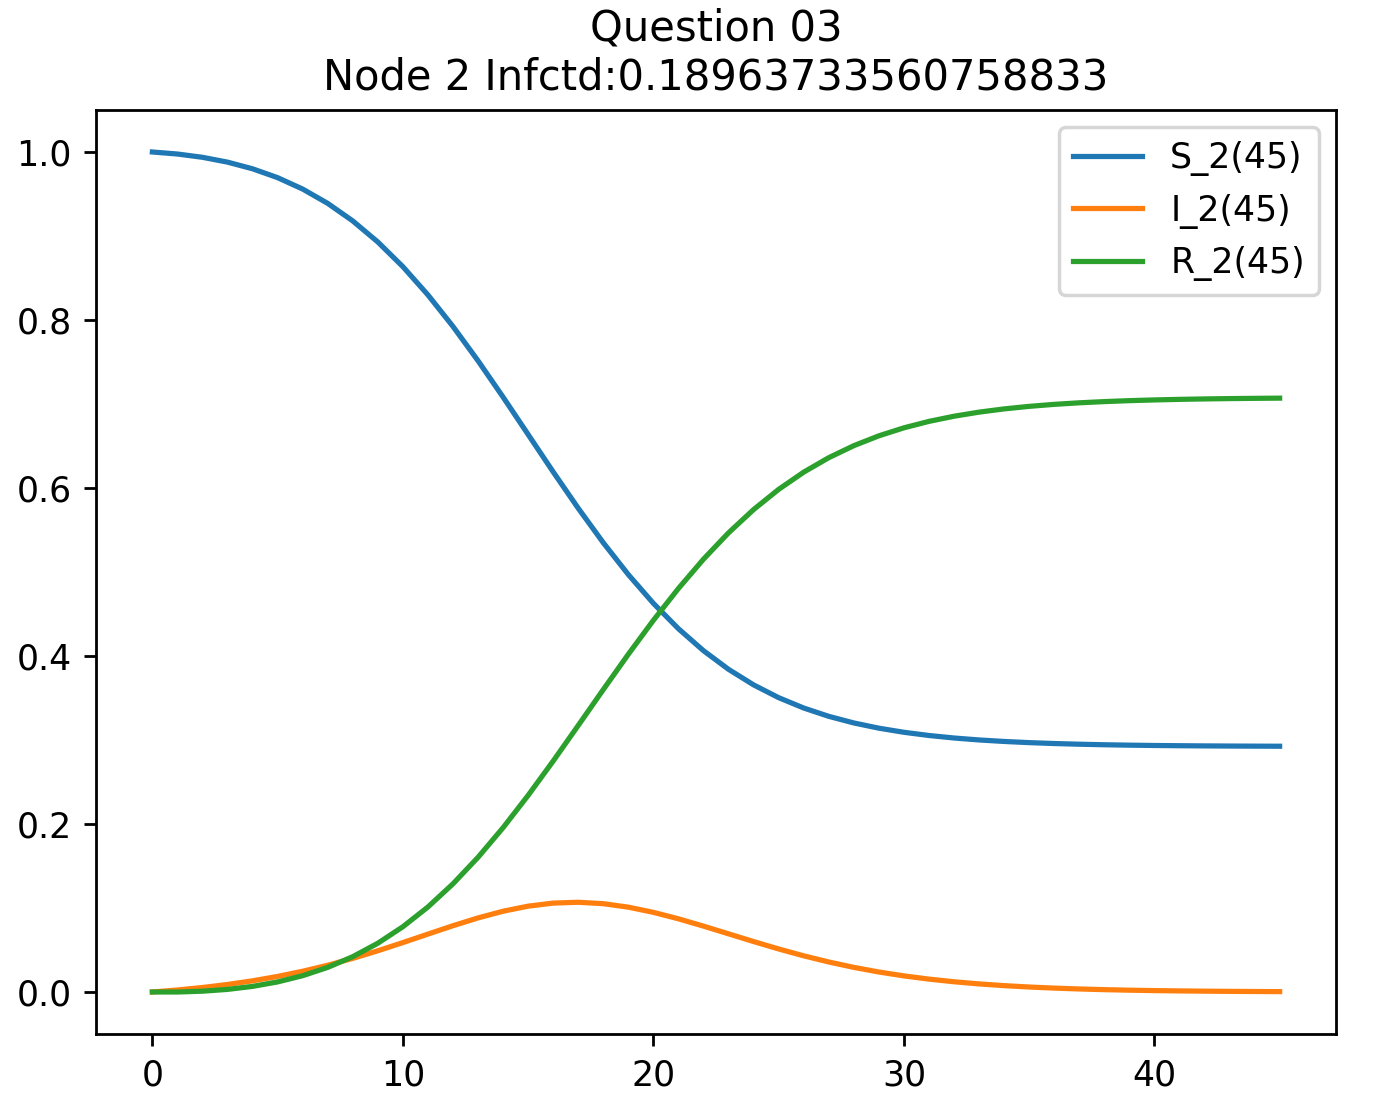
\includegraphics[scale=0.8]{Figure1.2}\\
	Figure 1.2
\end{center}
\end{enumerate}
}

% Question 4
\begin{enumerate}
	\setcounter{enumi}{3}
	\item Repeat that same thought experiment, but this time let the initial infection start on node 2 (so $I_2(0) = 0.01$ and $S_2(0) = 0.99$, but all other nodes have $S_i(0)=1$, $I_i(0)=0$  and $R_i(0)=0$). Now can you predict how many people in node 2 would eventually get sick?
\end{enumerate}
% Question 4 Answers
\textcolor{gray}{
Answers:
\begin{enumerate}
	\setcounter{enumi}{3}
	\item Repeat that same thought experiment, but this time let the initial infection start on node 2 (so $I_2(0) = 0.01$ and $S_2(0) = 0.99$, but all other nodes have $S_i(0)=1$, $I_i(0)=0$  and $R_i(0)=0$). Now can you predict how many people in node 2 would eventually get sick?
\end{enumerate}
}

% Question 5
\begin{enumerate}
	\setcounter{enumi}{4}
	\item Instead, suppose you remove the connection from node 2 to node 1, and replace it with a self-loop on 2 with weight 1. If nothing else changes in the network (and the infection starts at node 1), would this change the spread of the epidemic? Can you predict how many people in node 2 would eventually get sick?
\end{enumerate}
% Question 5 Answers
\textcolor{gray}{
Answers:
\begin{enumerate}
	\setcounter{enumi}{4}
	\item Instead, suppose you remove the connection from node 2 to node 1, and replace it with a self-loop on 2 with weight 1. If nothing else changes in the network (and the infection starts at node 1), would this change the spread of the epidemic? Can you predict how many people in node 2 would eventually get sick?
\end{enumerate}
}
\end{document}
